\begin{tcolorbox}[enhanced jigsaw,breakable,pad at break*=1mm,
    colback=blue!5!white,colframe=babyblueeyes,title=Exercises]
    Exercises may be the most important part of this module container.
    We suggest that you do them actively and in small groups. Really, the only way to learn Python is to do it.      
\end{tcolorbox}
\section{Exercises 0: Getting ready}

\subsection{Installation and development environment}
Python is an open-source environment with significant input from the user community.
Many of the developments are packaged in libraries designed for specific tasks.
These need to be installed prior to usage which at times can be a bit tricky because of dependencies between
different libraries. In order to alleviate you from installation difficulties that we have experienced in
the past, we provide a fully installed python environment in a virtual environment that can be run on any laptop.
If you use your own Laptop for the course this can be useful. Follow these steps to download and run the environment on your own computer:\\

\begin{enumerate}
    \item Download and install VirtualBox for your System: \url{https://www.virtualbox.org/}
    \item Copy the virtual machine files onto your system (external hard drive).
    \item Run VirtualBox and select $Machine \rightarrow Add$ from the menu.
    \item The virtual machine (vm) is now available on your system. You can start it by selecting the vm on the left side and click on the start button on the top right.
\end{enumerate}

\begin{figure}[h!]
    \centering
    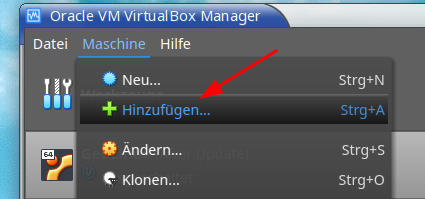
\includegraphics[width=8cm]{Figures/virtual_box1.png}
    \caption{Add a virtual machine to VirtualBox}
\end{figure}

\begin{figure}[h!]
    \centering
    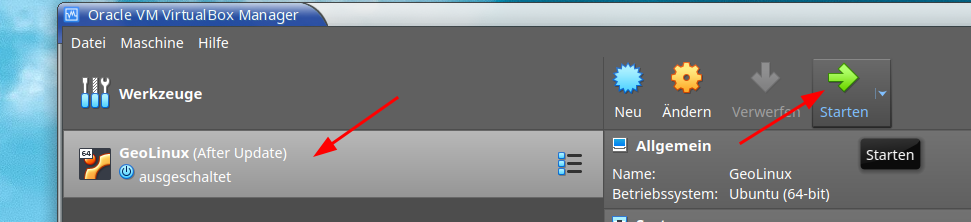
\includegraphics[width=10cm]{Figures/virtual_box2.png}
    \caption{Start the virtual machine}
\end{figure}

\vspace{1cm}

It is best if you do that BEFORE the first class, then we can hit the road running. If you prefer to run your own installation (let's say with Anaconda),
feel free to do it. Required packages are:

\begin{itemize}
    \item Matplotlib
    \item Numpy
    \item Pandas
\end{itemize}

In Order to verify that Python is working correctly you can try to run the following example:

\vspace{1cm}

\begin{tcolorbox}[enhanced jigsaw,breakable,pad at break*=1mm,
    colback=blue!5!white,colframe=babyblueeyes,title=Solutions,
    watermark color=white]
    Test Python environment
    \lstinputlisting[language=Python]{Src/Ex0/PlotExample.py}
\end{tcolorbox}

%\vspace{1cm}
\newpage

And this is what it should look like:

\vspace{1cm}

\begin{figure}[h!]
    \centering
    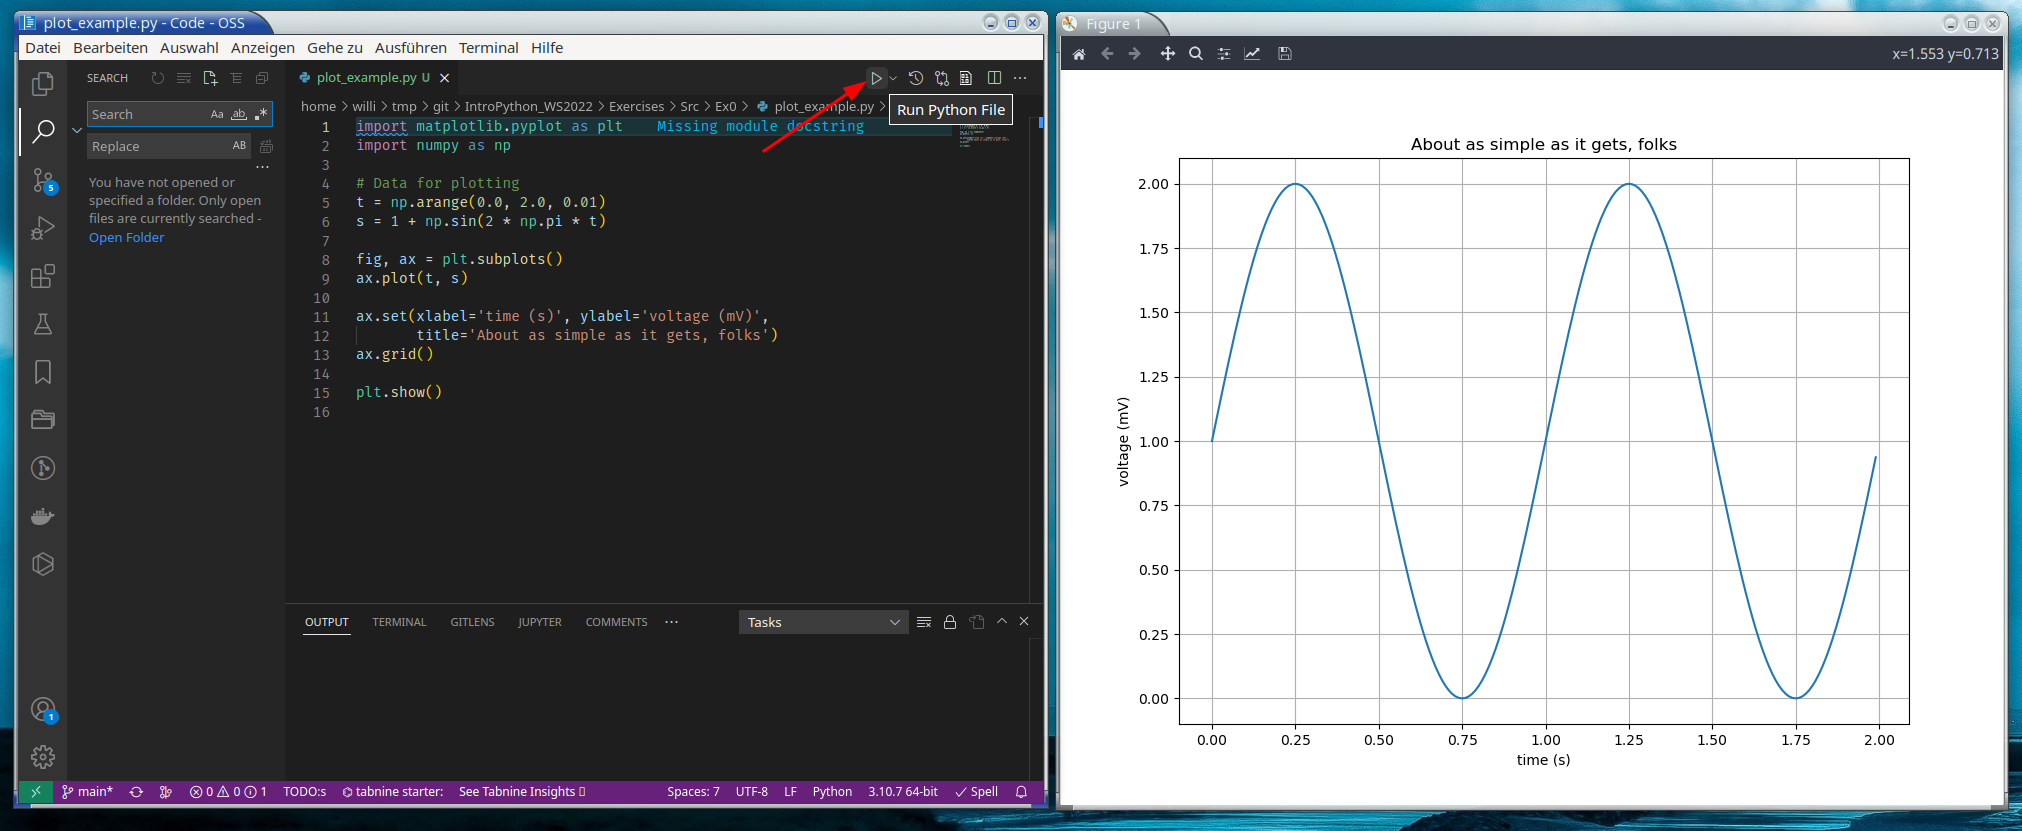
\includegraphics[width=18cm]{Figures/vs_code1.png}
    \caption{Test your Python environment}
\end{figure}

%\ifanswers
%    \begin{tcolorbox}[enhanced jigsaw,breakable,pad at break*=1mm,
%    colback=blue!5!white,colframe=babyblueeyes,title=Solutions,
%    watermark color=white]
%    test 
%    \lstinputlisting[language=Python]{Src/Ex1/HelloWorld.py}
%    \end{tcolorbox}
%\fi
